\documentclass[11pt,a4paper]{article}

\usepackage[T1]{fontenc}
\usepackage[utf8]{inputenc}
\usepackage{lmodern}
\usepackage{microtype}
\usepackage[margin=2.2cm]{geometry}
\usepackage{graphicx}
\usepackage{booktabs}
\usepackage{tabularx}
\usepackage{longtable}
\usepackage{array}
\usepackage{float}
\usepackage[font=small,labelfont=bf]{caption}
\usepackage{enumitem}
\usepackage{xcolor}
\usepackage{listings}
\usepackage{amsmath}
\usepackage{seqsplit}
\usepackage[hidelinks]{hyperref}

\definecolor{codebg}{RGB}{246,248,250}
\lstset{
  basicstyle=\ttfamily\small,
  backgroundcolor=\color{codebg},
  frame=single, rulecolor=\color{black!15},
  breaklines=true, columns=fullflexible,
  keepspaces=true, showstringspaces=false,
  xleftmargin=2pt, xrightmargin=2pt
}
\setlist{itemsep=2pt, topsep=4pt}
\setlength{\emergencystretch}{3em}
\newcommand{\file}[1]{\texttt{#1}}
\graphicspath{{figures/}}

\begin{document}

% ------------------------------------------------------------------ title
\begin{titlepage}
\centering
\vspace*{3cm}
{\LARGE\bfseries NoSQL Systems (DAS 838)\par}
\vspace{0.6cm}
{\Large Assignment 1\par}
\vspace{0.3cm}
{\large Data Scaling, Data Integration and Unix Data Processing\par}
\vspace{0.8cm}
{\large Instructor: Vinu E.\ Venugopal\par}
\vspace{2cm}
{\large\bfseries Team ID: 18, 28\par}
\vspace{0.6cm}
\begin{tabular}{ll}
\toprule
\textbf{Name} & \textbf{Roll number} \\
\midrule
Kalpit & BT2024093 \\
Cheruku Sri Charan Reddy & BT2024143 \\
Arnav Jain & BT2024233 \\
D Sree Teja & BT2024160 \\
\bottomrule
\end{tabular}
\vfill
{\large 15 September 2026\par}
\end{titlepage}

\tableofcontents
\newpage

% ------------------------------------------------------------------ intro
\section*{About this report}
\addcontentsline{toc}{section}{About this report}

This report covers all three problems of the assignment. For each one we
describe what we built, how we tested it, what we measured and what we think
the results mean. We have tried to back every number with a file in the
submission, and to say so openly where something did not work out or where
we could not find the cause of a result.

The submission folder mirrors the report: \file{problem1\_tpch/},
\file{problem2\_integration/} and \file{problem3\_unix\_pipeline/} each contain
the code, the inputs, the raw outputs and a README with the same material in
more detail. \file{COMPLIANCE.md} lists every requirement from the assignment
PDF next to the file that addresses it; Section~\ref{sec:compliance} gives a
short version of it.

\paragraph{Use of AI tools.} As the assignment allows, we used an AI coding
assistant (Claude Code) for help with writing and debugging scripts, reviewing
our results against the assignment and drafting documentation. The experiments
were run by us on the machines described below, and every number in this
report comes from the output files included in the submission, so it can be
checked and reproduced.

\paragraph{Machines.} Problem~1 ran on a lab server with an Intel Core
i9-12900K (16 cores, 24 threads), 62\,GB of RAM and an NVMe SSD, under Red Hat
Enterprise Linux 8.10. Problems~2 and~3 ran on a laptop with an AMD Ryzen~7
5800H (8 cores, 16 threads), 16\,GB of RAM and an NVMe SSD, under Windows~11
with Git Bash (GNU awk 5.4.0, GNU coreutils 8.32) and Python 3.12.10.

% ================================================================== P1
\section{Scaling study with the TPC-H benchmark}
\label{sec:p1}

\subsection{What we set out to do}

The task was to run the TPC-H decision-support queries on a growing dataset,
doubling the scale factor each time, and to work out how query time responds
to the extra data. We used PostgreSQL, as the assignment suggests, and went
from scale factor 1 up to 32.

We should mention that this is our second attempt. The first run used a
copy of the TPC-H tools from GitHub (version 2.14) and generated the queries
only once. That turned out to be a problem for Q11, whose threshold is
supposed to shrink with the scale factor, so we threw those numbers away and
repeated the whole study with the official kit and per-scale query
generation. Everything below comes from the second run.

\subsection{Experimental setup}

\begin{table}[H]
\centering
\small
\begin{tabularx}{\textwidth}{@{}lX@{}}
\toprule
Benchmark & Official TPC-H Tools v3.0.1 from tpc.org
(\texttt{\seqsplit{7C5384AF-10DA-4DCB-B83F-BA2BDE51003F-TPC-H-Tool.zip}}), SHA-256
\texttt{\seqsplit{97ccb34cd122d78c2e06e2419e50957f934256868b37c02d0b88aefd9d13a84a}} \\
Tool banners & \file{dbgen}: ``Version 3.0.0 build 0'', \file{qgen}:
``v.~3.0.0 build 0'' (this is what the programs in the 3.0.1 kit print) \\
Database & PostgreSQL 16.15, compiled from source, one build for all runs \\
Hardware & Intel Core i9-12900K, 62\,GB RAM, 931.5\,GB NVMe SSD (Crucial CT1000P3SSD8) \\
OS, compiler & Red Hat Enterprise Linux 8.10 (kernel 4.18), gcc 8.5.0 \\
Scale factors & 1, 2, 4, 8, 16, 32 \\
Queries & all 22, generated separately for every scale factor with
\file{qgen -r 42 -s <SF>} \\
Repetitions & one warm-up run (not counted) and three measured runs per query \\
Timeout & 30 minutes per query at every scale factor (never reached) \\
\bottomrule
\end{tabularx}
\caption{Experimental setup for Problem 1.}
\end{table}

The PostgreSQL settings were fixed before the first run and never touched
afterwards. The database cluster was created with the C locale, which
matters for the answer check described below.

\begin{lstlisting}
shared_buffers = 4GB              effective_cache_size = 12GB
work_mem = 128MB                  maintenance_work_mem = 1GB
max_parallel_workers_per_gather = 4
random_page_cost = 1.1            max_wal_size = 8GB
jit = off                         synchronous_commit = on
\end{lstlisting}

On top of the TPC-H schema we created primary keys on all eight tables,
indexes on the foreign-key columns, and indexes on \file{l\_shipdate} and
\file{o\_orderdate}. They are built after loading, the same way at every
scale.

We ran SF1 to SF16 in one go and SF32 in a second session later the same
day, because the disk on the server is shared and we had to free space in
between. Both sessions recorded their environment in
\file{results/environment.txt}. Apart from the date, the load average and the
free memory and disk, the two records are identical. The load average of the
machine (24 logical CPUs) was 3.74 when the first session started and 0.08
when the second one started.

\subsection{How the runs were done}

The whole procedure is in \file{run\_benchmark.sh}. For every scale factor it
does the following.

\begin{enumerate}
\item \textbf{Generate the queries.} \file{qgen} writes the 22 queries for
that scale factor. We keep its exact output and a PostgreSQL version of each
query, with SHA-256 checksums for both. The kit has no PostgreSQL output
mode, so we built \file{qgen} for Oracle and changed two things afterwards:
the row limit (\file{where rownum <= N}) becomes \file{LIMIT N}, and the
\file{day (3)} precision in Q1's interval is dropped because PostgreSQL does
not accept it. Scale-dependent parameters come straight from \file{qgen}; for
example the Q11 threshold is 0.0001 at SF1 and 0.000003125 at SF32.
\item \textbf{Generate and load the data.} \file{dbgen -s <SF>} produces the
eight tables, which are streamed into PostgreSQL with \file{COPY}. After
loading, the script compares the number of rows in each table with the number
of lines \file{dbgen} produced and stops if they differ. They matched for all
48 table and scale combinations, for example 6{,}001{,}215 \file{lineitem}
rows at SF1 and 192{,}000{,}551 at SF32.
\item \textbf{Index and analyse.} The indexes are built and
\file{VACUUM ANALYZE} is run. The load time and the database size are
recorded.
\item \textbf{Check correctness (SF1 only).} The kit comes with official
answers for SF1, computed with default query parameters. We generated that
query set with \file{qgen -d}, ran it, and compared the results using the
tolerances from the kit's own checker. All 22 queries passed, and the kit's
checker script \file{cmpq.pl} reports zero unacceptable mismatches as well.
The only value that is not identical is Q17 (official 348406.02, ours
348406.05). It is an average, for which the specification allows a
difference of up to one percent.
\item \textbf{Save the plans.} The \file{EXPLAIN} output of every query is
stored, so we can see later which join and scan methods PostgreSQL chose.
\item \textbf{Time the queries.} Each query runs once as a warm-up and then
three more times. We record the wall-clock time around \file{psql}
(connection and result transfer included) and whether the query succeeded.
\end{enumerate}

All 528 query executions (6 scale factors $\times$ 22 queries $\times$ 4 runs)
completed successfully. We use the median of the three measured runs.

\subsection{Reproducing the study}

These are the exact commands we used. The first one builds PostgreSQL and the
TPC-H tools in the user's home directory and needs no administrator rights.
Generating the data is part of \file{run\_benchmark.sh} (it calls
\file{dbgen -s <SF>} for each scale factor, see step~2 above).

\begin{lstlisting}
cd problem1_tpch
TPCH_KIT=/path/to/7C5384AF-10DA-4DCB-B83F-BA2BDE51003F-TPC-H-Tool.zip \
  ROOT=$HOME/nosql_a1 bash setup_postgres_and_dbgen.sh
source $HOME/nosql_a1/env.sh
bash run_benchmark.sh 1 2 4 8 16      # first session
bash run_benchmark.sh 32              # second session
python3 plot_results.py               # tables and plots
\end{lstlisting}

To check a single query set against its recorded checksums:
\file{cd queries/sf32 \&\& sha256sum -c SHA256SUMS}.

\subsection{Results}

\begin{table}[H]
\centering
\small
\begin{tabular}{@{}rrrrrrrrr@{}}
\toprule
SF & Raw data & DB size & Load+index & Run 1 & Run 2 & Run 3 & Median & $\times$ prev. \\
   & (MB) & (MB) & (s) & (s) & (s) & (s) & (s) & \\
\midrule
1  & 1{,}049.7  & 1{,}704.4  & 18.4  & 6.23   & 6.16   & 6.31   & \textbf{6.23}   & -- \\
2  & 2{,}114.6  & 3{,}397.7  & 38.1  & 16.41  & 15.08  & 13.84  & \textbf{15.08}  & 2.42 \\
4  & 4{,}254.5  & 6{,}783.8  & 83.2  & 36.48  & 38.15  & 37.05  & \textbf{37.05}  & 2.46 \\
8  & 8{,}555.8  & 13{,}555.6 & 155.4 & 69.48  & 63.63  & 60.50  & \textbf{63.63}  & 1.72 \\
16 & 17{,}220.6 & 27{,}102.6 & 308.4 & 121.70 & 123.07 & 122.74 & \textbf{122.74} & 1.93 \\
32 & 34{,}688.3 & 54{,}197.3 & 636.1 & 354.27 & 316.77 & 328.23 & \textbf{328.23} & 2.67 \\
\bottomrule
\end{tabular}
\caption{Dataset size, load time and total time of the 22 queries at each scale factor.}
\label{tab:totals}
\end{table}

\begin{table}[H]
\centering
\footnotesize
\setlength{\tabcolsep}{3.6pt}
\begin{tabular}{@{}lrrrrrrrrrrrr@{}}
\toprule
 & \multicolumn{6}{c}{Median time (s)} & \multicolumn{5}{c}{Ratio at each doubling} & \\
\cmidrule(lr){2-7}\cmidrule(lr){8-12}
Query & SF1 & SF2 & SF4 & SF8 & SF16 & SF32 & 2/1 & 4/2 & 8/4 & 16/8 & 32/16 & Slope \\
\midrule
Q1  & 0.65 & 1.32 & 2.70  & 5.29  & 10.42 & 20.85 & 2.04 & 2.03 & 1.96 & 1.97 & 2.00 & 0.99 \\
Q2  & 0.12 & 0.28 & 0.88  & 1.69  & 3.10  & 6.98  & 2.45 & \textbf{3.12} & 1.92 & 1.83 & 2.25 & 1.16 \\
Q3  & 0.22 & 0.49 & 1.11  & 2.00  & 2.56  & 5.73  & 2.23 & 2.29 & 1.80 & \textbf{1.28} & 2.24 & 0.90 \\
Q4  & 0.06 & 0.12 & 0.29  & 0.57  & 1.30  & 2.54  & 1.92 & 2.45 & 1.96 & 2.28 & 1.95 & 1.08 \\
Q5  & 0.13 & 0.31 & 0.64  & 0.99  & 1.70  & 6.52  & 2.39 & 2.06 & 1.56 & 1.71 & \textbf{3.85} & 1.03 \\
Q6  & 0.12 & 0.27 & 0.67  & 1.39  & 2.76  & 2.90  & 2.15 & 2.51 & 2.08 & 1.99 & \textbf{1.05} & 0.96 \\
Q7  & 0.34 & 0.92 & 3.10  & 4.00  & 6.30  & 15.87 & 2.75 & \textbf{3.36} & \textbf{1.29} & 1.58 & 2.52 & 1.03 \\
Q8  & 0.08 & 0.18 & 0.40  & 0.66  & 1.92  & 2.60  & 2.10 & 2.27 & 1.65 & 2.91 & \textbf{1.36} & 1.01 \\
Q9  & 0.49 & 1.14 & 2.26  & 5.84  & 9.28  & 29.86 & 2.31 & 1.98 & 2.59 & 1.59 & \textbf{3.22} & 1.13 \\
Q10 & 0.11 & 0.30 & 0.66  & 1.27  & 2.34  & 7.28  & 2.68 & 2.18 & 1.92 & 1.84 & \textbf{3.11} & 1.13 \\
Q11 & 0.05 & 0.13 & 0.42  & 0.72  & 1.25  & 2.83  & 2.48 & \textbf{3.28} & 1.70 & 1.74 & 2.26 & 1.12 \\
Q12 & 0.15 & 0.32 & 0.77  & 1.36  & 2.48  & 5.67  & 2.18 & 2.38 & 1.77 & 1.82 & 2.28 & 1.02 \\
Q13 & 0.47 & 1.32 & 3.76  & 7.46  & 13.55 & 62.04 & 2.81 & 2.85 & 1.98 & 1.82 & \textbf{4.58} & 1.31 \\
Q14 & 0.05 & 0.11 & 0.26  & 0.55  & 1.09  & 2.24  & 2.00 & 2.44 & 2.11 & 2.00 & 2.05 & 1.08 \\
Q15 & 0.25 & 0.59 & 1.53  & 4.31  & 8.30  & 8.75  & 2.39 & 2.61 & 2.81 & 1.93 & \textbf{1.05} & 1.10 \\
Q16 & 0.10 & 0.18 & 0.39  & 0.63  & 1.29  & 8.51  & 1.88 & 2.15 & 1.62 & 2.06 & \textbf{6.61} & 1.18 \\
Q17 & 0.37 & 0.96 & 2.15  & 3.66  & 7.59  & 15.66 & 2.63 & 2.23 & 1.70 & 2.08 & 2.06 & 1.04 \\
Q18 & 1.78 & 4.36 & 11.64 & 12.22 & 26.46 & 57.21 & 2.45 & 2.67 & \textbf{1.05} & 2.16 & 2.16 & 0.93 \\
Q19 & 0.03 & 0.06 & 0.09  & 0.14  & 0.28  & 1.08  & 2.04 & 1.62 & 1.52 & 2.04 & \textbf{3.92} & 0.97 \\
Q20 & 0.33 & 0.68 & 1.51  & 6.21  & 13.32 & 42.28 & 2.09 & 2.22 & \textbf{4.12} & 2.14 & \textbf{3.17} & 1.42 \\
Q21 & 0.28 & 0.60 & 1.91  & 2.32  & 5.26  & 10.82 & 2.19 & \textbf{3.18} & \textbf{1.22} & 2.26 & 2.06 & 1.02 \\
Q22 & 0.03 & 0.06 & 0.12  & 0.19  & 0.36  & 0.72  & 1.82 & 1.90 & 1.58 & 1.94 & 1.98 & 0.86 \\
\bottomrule
\end{tabular}
\caption{Median time per query and the ratio between consecutive scale
factors. A ratio of 2 means the time doubled along with the data. Ratios of 3
or more and of 1.4 or less are in bold. The slope is fitted to log(time)
against log(dataset size) over all six scale factors, so 1 means linear
growth.}
\label{tab:perquery}
\end{table}

\begin{figure}[H]
\centering
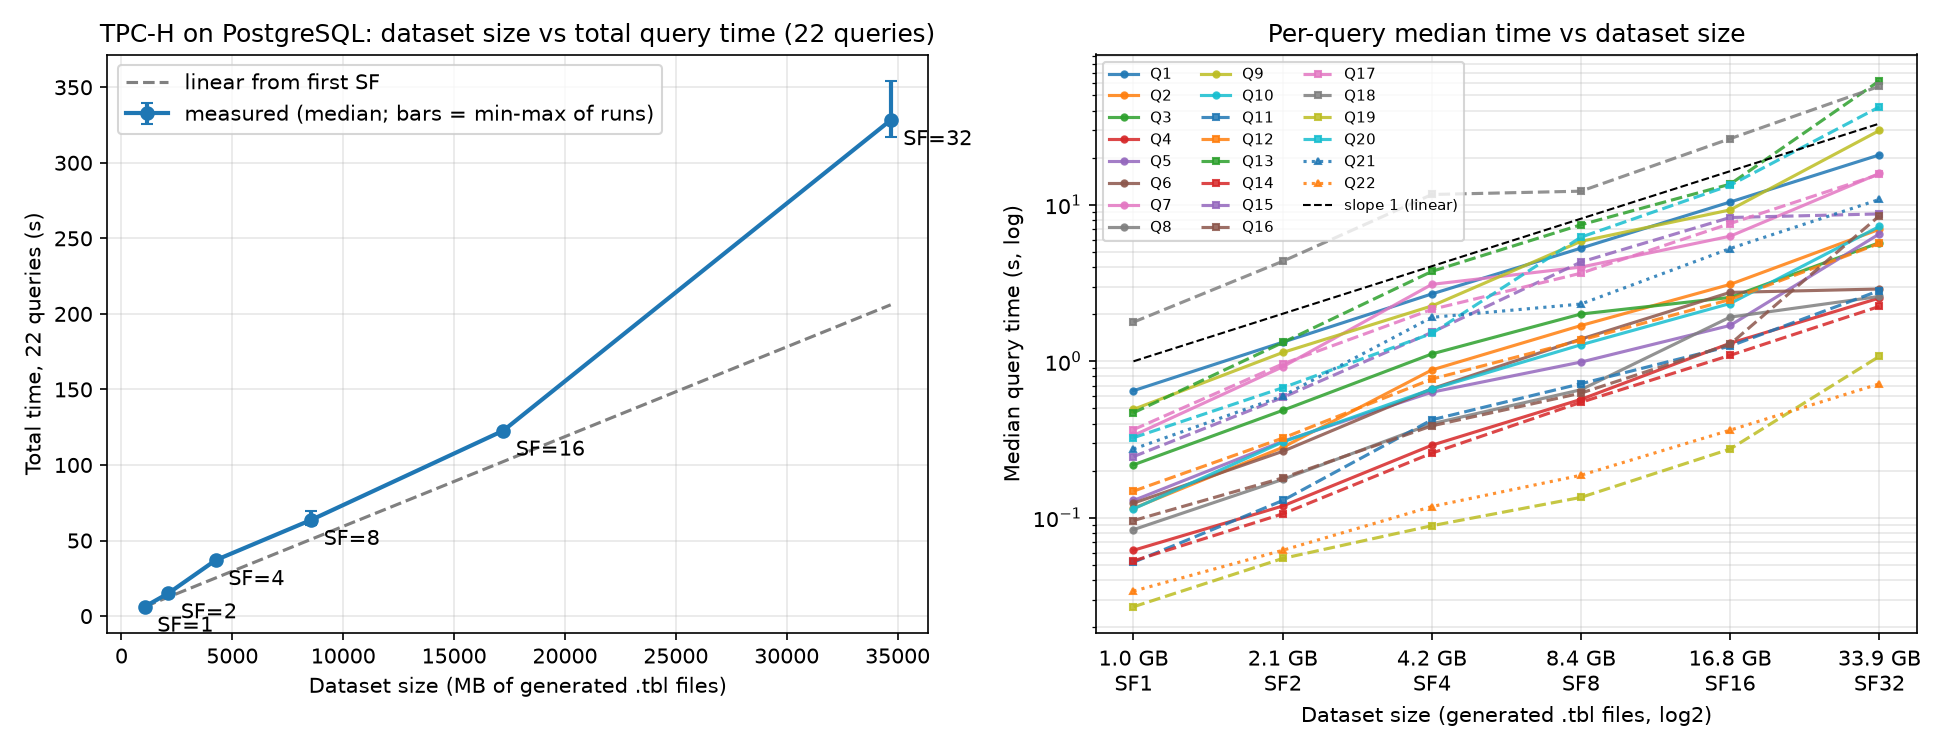
\includegraphics[width=\textwidth]{scaling_plot.png}
\caption{Left: total time of the 22 queries against dataset size, with the
spread of the three runs and a line for purely linear growth from SF1.
Right: median time of each query against dataset size on log--log axes.}
\label{fig:scaling}
\end{figure}

\begin{figure}[H]
\centering
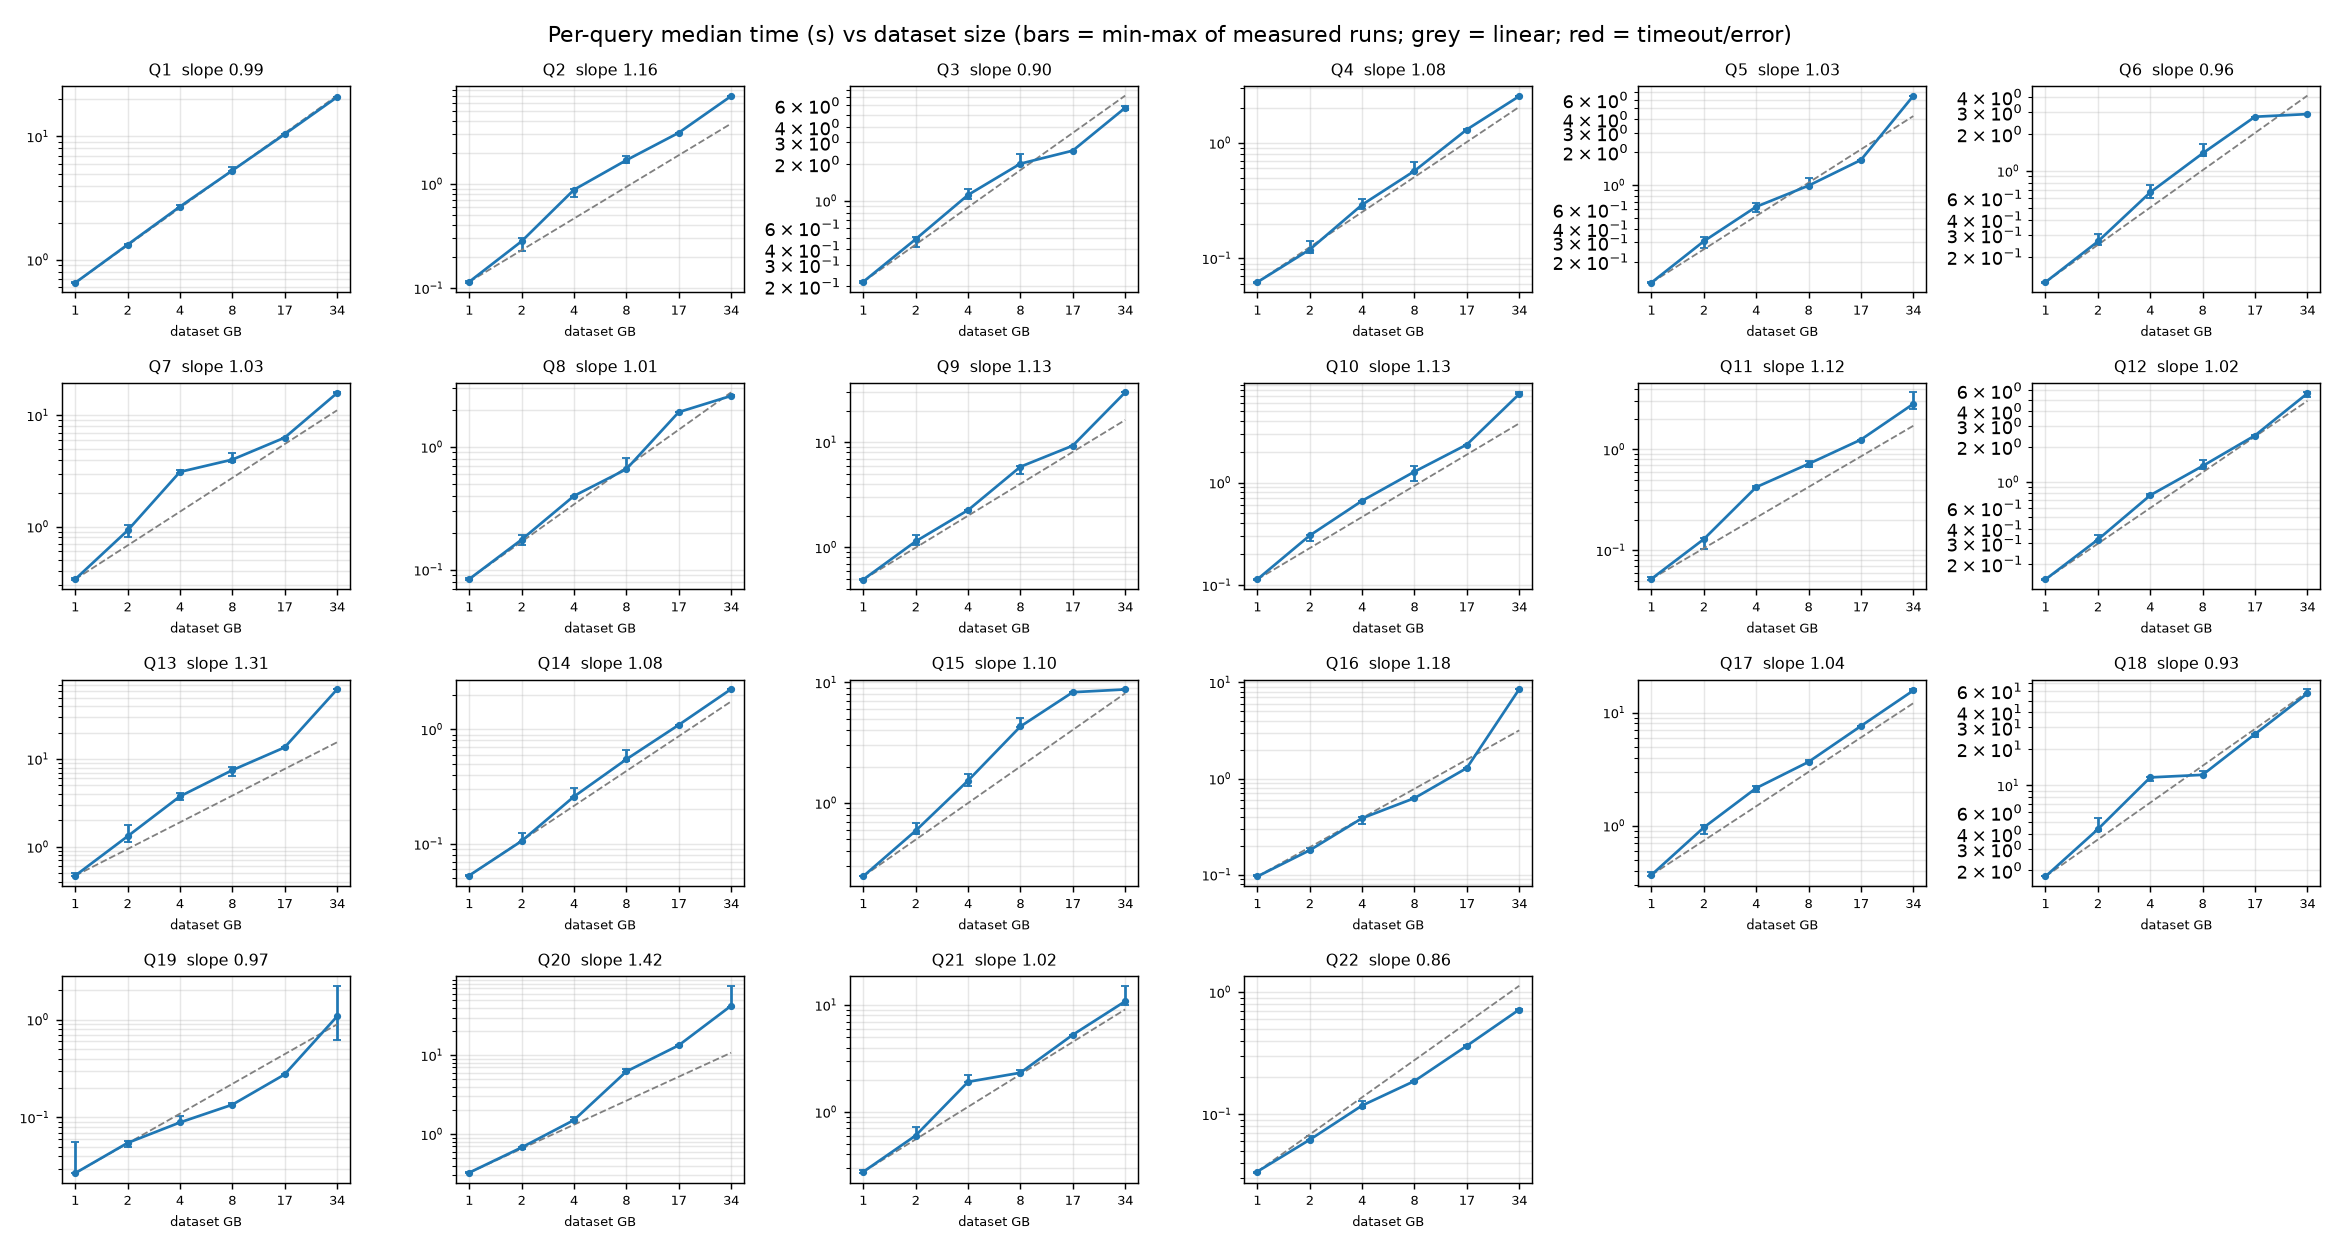
\includegraphics[width=\textwidth]{per_query_plot.png}
\caption{One panel per query. The grey line is linear growth from SF1; the
bars show the minimum and maximum of the three measured runs.}
\label{fig:perquery}
\end{figure}

\subsection{Answers to the assignment's questions}

The assignment asks five questions about the scaling behaviour. Here are our
short answers; the following subsections give the evidence.

\begin{enumerate}[label=\textbf{(\arabic*)}, leftmargin=2.2em]
\item \textbf{Does query time approximately double when the dataset doubles?}
Up to SF16, roughly yes: the total time grows by 2.42, 2.46, 1.72 and 1.93 at
the first four doublings (with some noise at SF2--SF8, see
Section~\ref{sec:p1reliability}). At the last doubling it grows by 2.67. Over
the whole range the data grows 33.0 times and the total time 52.7 times, which
corresponds to time $\propto$ size$^{1.13}$, slightly worse than linear.
Loading and indexing, in contrast, double almost exactly (1.87--2.19 per step).

\item \textbf{Which queries show linear and which super-linear scaling?}
\emph{Linear:} Q1, Q4, Q12, Q14 and Q17. Every ratio lies between 1.70 and
2.63, the fitted slopes are 0.99--1.08, and their plans never change. Q1 is
the clearest case: 32.1 times slower for 33.0 times more data.
\emph{Super-linear over the whole range:} Q20 (slope 1.42), Q13 (1.31), Q16
(1.18) and Q2 (1.16). \emph{Super-linear at a single step:} seven queries
become more than three times slower from SF16 to SF32 (Q16, Q13, Q19, Q5, Q9,
Q20, Q10), Q20 also from SF4 to SF8, and Q2, Q7, Q11 and Q21 from SF2 to SF4.

\item \textbf{Which queries are relatively insensitive to dataset size?}
None over the whole range; every query is at least 21 times slower at SF32
than at SF1. The least sensitive is Q22 (21.1 times for 33.0 times the data,
slope 0.86), because it takes only a few hundredths of a second and part of
that is the fixed cost of starting \file{psql}. Some queries look insensitive
for a single step: Q6 and Q15 from SF16 to SF32 (1.05) and Q18 from SF4 to SF8
(1.05). Each of these coincides with a plan change, and they grow again at the
next doubling.

\item \textbf{At what scale factor does performance begin to degrade
significantly?} At SF32. The total grows by 2.67 there, the most of any step,
and seven queries become more than three times slower in that one doubling.
At that scale the database (54.2\,GB) approaches the machine's 62\,GB of RAM,
and the \file{EXPLAIN ANALYZE} plans show random index access and sorts and
aggregations spilling to disk. A single query, Q20, already degrades at SF8,
when its plan switches to running a subquery per row.

\item \textbf{How do the observations relate to joins, aggregation, sorting
and filtering?} Filtering and scanning scale linearly. Aggregation stays
linear while its hash table fits in memory (Q1) and becomes much slower once
it spills to disk (Q18 at SF32). Sorting is negligible for small results but
turns into external merge sorts on disk when the input exceeds
\file{work\_mem} (Q16, Q9, Q10 at SF32). Joins cause most of the irregular
behaviour, because the planner switches between index nested loops, hash
joins and merge joins as the tables grow (Q3, Q5, Q10, Q13, Q20). Details are
in Table~\ref{tab:operations}.
\end{enumerate}

\subsection{What the numbers tell us}

\subsubsection*{Does the time double when the data doubles?}

Roughly, but not exactly, and not for every query. Between SF1 and SF32 the
data grew by a factor of 33.0 and the total query time by a factor of 52.7,
so the workload as a whole got slower a bit faster than the data grew. The
ratio for the total stayed between 1.72 and 2.46 up to SF16 and then jumped
to 2.67 at SF32, the highest of all the steps. Loading and indexing, on the
other hand, scaled almost perfectly (ratios 2.07, 2.19, 1.87, 1.98 and 2.06),
so the extra cost is not in reading more data but in how the queries are
executed. Looking at the queries one by one, we found three different
patterns.

\subsubsection*{Queries that scale linearly}

Q1, Q4, Q12, Q14 and Q17 grow steadily: every ratio lies between 1.70 and
2.63, and their slopes are between 0.99 and 1.08. When we compared their saved
plans, we noticed that PostgreSQL used the same plan shape for these queries
at all six scale factors, which explains why their cost simply follows the
number of rows.

Q1 is the clearest example, with ratios between 1.96 and 2.04. It filters
\file{lineitem} on the ship date and groups the result into four groups. At
SF32 the plan is a parallel sequential scan in five processes that returns
189 million of the 192 million rows; the aggregation needs only 24\,kB of
memory per process and the final sort 27\,kB. The work is essentially reading
every row once, so the time doubles with the data. Q12 and Q14 are similar
filter-join-aggregate queries. Q17 is interesting because it contains a
correlated subquery, yet it still scales linearly. Its plan does not change,
which shows that a subquery on its own does not make a query super-linear.

Q22 grows a little more slowly than the data (slope 0.86). It is also the
fastest query, at 0.03\,s for SF1, and our timing includes starting
\file{psql}, a fixed cost that does not depend on the data. For such a short
query that fixed part is a noticeable share of the measurement.

\subsubsection*{Steps caused by the planner changing its mind}

Several of the odd ratios in Table~\ref{tab:perquery} line up exactly with a
change in the saved plans between two scale factors.

\begin{table}[H]
\centering
\small
\begin{tabularx}{\textwidth}{@{}llX@{}}
\toprule
Query, step & Ratio & Plan at the smaller scale $\rightarrow$ plan at the larger scale \\
\midrule
Q6, SF16$\rightarrow$32  & 1.05 & bitmap scan on the \file{l\_shipdate} index $\rightarrow$ parallel sequential scan \\
Q15, SF16$\rightarrow$32 & 1.05 & serial aggregation $\rightarrow$ parallel aggregation \\
Q18, SF4$\rightarrow$8   & 1.05 & serial hash aggregation $\rightarrow$ parallel partial hash aggregation \\
Q21, SF4$\rightarrow$8   & 1.22 & different join order and access paths \\
Q3, SF8$\rightarrow$16   & 1.28 & nested loops with index lookups $\rightarrow$ parallel hash joins \\
Q7, SF4$\rightarrow$8    & 1.29 & ordinary hash joins $\rightarrow$ parallel hash join with partial aggregation \\
Q8, SF16$\rightarrow$32  & 1.36 & more of the joins become parallel hash joins \\
Q20, SF4$\rightarrow$8   & 4.12 & hash semi-join $\rightarrow$ nested-loop semi-join running a subquery per row \\
Q5, SF16$\rightarrow$32  & 3.85 & index lookups into \file{lineitem} $\rightarrow$ parallel scan of \file{lineitem} and hash joins \\
Q10, SF16$\rightarrow$32 & 3.11 & index lookups into \file{lineitem} $\rightarrow$ parallel scan of \file{lineitem} and hash join \\
\bottomrule
\end{tabularx}
\caption{Scaling steps that coincide with a plan change.}
\end{table}

PostgreSQL picks plans by estimated cost. With small tables an index lookup
is cheap; once many rows qualify, a sequential scan, a hash join or parallel
workers become cheaper. When that switch pays off, the step looks almost flat
(Q6, Q15, Q18, Q3). When the new plan does more work per row, the step is
steep (Q20, Q5, Q10). So the flat steps do not mean a query is insensitive to
the dataset size: they are one-off switches, and at the next doubling the time
grows again (Q18 goes from 1.05 to 2.16, Q7 from 1.29 to 1.58 to 2.52, Q3 from
1.28 to 2.24). None of the 22 queries is insensitive to the data size over the
whole range.

\subsubsection*{Where performance starts to degrade}

The clearest degradation happens at SF32. The total grows by 2.67 there, and
seven queries become more than three times slower in that one step: Q16
(6.61), Q13 (4.58), Q19 (3.92), Q5 (3.85), Q9 (3.22), Q20 (3.17) and Q10
(3.11). At this scale the database takes 54.2\,GB, close to the 62\,GB of RAM
on the machine, while PostgreSQL's own cache is set to 4\,GB. To see where the
time goes, we ran \file{EXPLAIN (ANALYZE, BUFFERS)} for these queries on the
SF32 database.

\begin{itemize}
\item \textbf{Q13} counts orders per customer with a left join. At SF16
PostgreSQL used a hash join over a sequential scan of \file{orders}. At SF32
it switched to a merge join that reads \file{orders} through the customer
index, which means reading the table in customer order instead of in the
order it is stored on disk. That index scan alone took 59.2 of the 65.2
seconds, with 18.4 million page reads outside PostgreSQL's cache.
\item \textbf{Q16} joins \file{part} with \file{partsupp} and counts distinct
suppliers. At SF16 the join ran in parallel. At SF32 the join is serial, and
sorting its result no longer fits into the 128\,MB of \file{work\_mem}, so
PostgreSQL falls back to an external merge sort that writes 193\,MB to
temporary files.
\item \textbf{Q9} is a six-table join. At SF32 its plan looks up
\file{lineitem} through an index 1{,}390{,}984 times and \file{orders} by
primary key 10{,}433{,}108 times, and each of its five parallel sorts spills
about 135\,MB to disk.
\item \textbf{Q5 and Q10} switched from index lookups into \file{lineitem} to
a parallel scan of the whole table joined against a large hash table built
from the other join input (350\,MB for Q5, 936\,MB for Q10). Q10's five
parallel sorts also write about 138\,MB each to disk.
\item \textbf{Q20} contains a correlated subquery. Since its plan change at
SF8, the subquery runs once for every candidate row of \file{partsupp}. At
SF32 that is 786{,}335 separate index lookups into \file{lineitem}. It has the
highest slope of all queries (1.42), and its three runs at SF32 took 75.7,
41.1 and 42.3 seconds, which fits a query that depends heavily on what happens
to be in the cache.
\item \textbf{Q18} groups \file{lineitem} by order. It scales linearly from
SF8 onwards, but at SF32 the hash table no longer fits in memory: the final
aggregation is split into 133 batches that use 4.0\,GB of temporary disk, and
each parallel worker writes about 1.3\,GB more. With 57.2\,s it is the second
slowest query at SF32, after Q13.
\item \textbf{Q19} kept the same plan but still grew by 3.92. Its times are
very small (0.28\,s to 1.08\,s) and its three runs at SF32 were 2.21, 1.08
and 0.61 seconds. With that much spread we do not want to claim a cause.
\end{itemize}

\subsubsection*{Relating this to joins, aggregation, sorting and filtering}

\begin{table}[H]
\centering
\small
\begin{tabularx}{\textwidth}{@{}p{2.6cm}XX@{}}
\toprule
Operation & What we observed & Where \\
\midrule
Filtering and scanning & Linear. Parallel sequential scans spread the work over five processes. & Q1, Q12, Q14; Q6 at SF32 \\
Aggregation & Linear while the hash table fits in \file{work\_mem}; much slower once it has to spill to disk in batches. & Q1 (4 groups, 24\,kB) against Q18 (133 batches, 4.0\,GB on disk at SF32) \\
Sorting & Negligible for small results; external merge sorts on disk once the input is larger than \file{work\_mem}. & Q16 (193\,MB), Q9 and Q10 (around 135--138\,MB per sort) at SF32 \\
Joins & The planner moves between index nested loops, hash joins and merge joins as the tables grow. These switches cause both the flat steps and the sudden jumps. & Q3, Q5, Q7, Q10, Q13, Q20, Q21 \\
Correlated subqueries & Cost is roughly outer rows times inner lookup; super-linear when the plan runs the subquery row by row. & Q20 (786{,}335 executions); Q17 stays linear \\
\bottomrule
\end{tabularx}
\caption{The observations grouped by database operation.}
\label{tab:operations}
\end{table}

\subsection{How reliable are the measurements?}
\label{sec:p1reliability}

Because the server is shared, we looked at how much the three measured runs
of the same query differ. For every query that takes at least half a second,
we computed the spread as (slowest $-$ fastest) / median.

\begin{table}[H]
\centering
\small
\begin{tabular}{@{}rrrrr@{}}
\toprule
SF & Queries $\geq$ 0.5\,s & Median spread & Largest spread & Spread of the total \\
\midrule
1  & 2  & 1.3\,\%  & 1\,\% (Q1)    & 2.4\,\% \\
2  & 9  & 23.0\,\% & 49\,\% (Q13)  & 17.1\,\% \\
4  & 15 & 12.7\,\% & 25\,\% (Q6)   & 4.5\,\% \\
8  & 20 & 18.2\,\% & 32\,\% (Q10)  & 14.1\,\% \\
16 & 20 & 0.5\,\%  & 5\,\% (Q18)   & 1.1\,\% \\
32 & 22 & 1.5\,\%  & 149\,\% (Q19) & 11.4\,\% \\
\bottomrule
\end{tabular}
\caption{Run-to-run spread of the three measured runs.}
\label{tab:spread}
\end{table}

The runs at SF1, SF16 and most of SF32 are very consistent. At SF2, SF4 and
SF8 the three runs of the same query differ by 13--23\,\% on a typical query,
so these scale factors were measured while the machine was busier (the load
average was 3.74 when that session started). This means that ratios involving
SF2, SF4 or SF8 are only accurate to roughly $\pm$20\,\%, and we do not read
anything into differences smaller than that. The main conclusions do not
depend on these steps: the linear queries are linear at every step, and the
degradation we describe happens at SF32, where the runs are consistent (apart
from Q19 and Q20, discussed above).

The three sharp increases from SF2 to SF4 that we could not explain from the
plans (Q2 3.12$\times$, Q11 3.28$\times$, Q21 3.18$\times$) are well above
this noise. Every single run is slower at SF4: Q11, for example, took
0.10--0.13\,s in all four runs at SF2 and 0.42--0.44\,s in all four runs at
SF4. So they are real effects, not measurement noise.

\subsection{Limitations}

\begin{itemize}
\item This is not an audited TPC-H result. We only measure single-stream
query times, we do not run the refresh functions or the throughput test, and
we added indexes. That is what the assignment asks for, but the numbers should
not be compared with published TPC-H results.
\item The server is shared with other users, and the SF2--SF8 measurements are
noticeably noisier than the others (Table~\ref{tab:spread}). We used the same
machine and configuration throughout, but we could not control what other
users were running.
\item Some jumps have no explanation in the plans. Q2 (3.12), Q11 (3.28) and
Q21 (3.18) grew quickly and consistently from SF2 to SF4 with the same plan
shape. Q19 grew by 3.92 at SF32, but its runs vary too much to be sure. We
report these without a cause.
\item We captured \file{EXPLAIN ANALYZE} only at SF32. For the smaller scales
we have the plain \file{EXPLAIN} plans, which show the chosen operators but
not the actual row counts or memory use.
\item SF32 was the largest scale we could run. It needs about 54\,GB for the
database and up to 34\,GB more for the raw files during loading, and the
shared disk had around 95\,GB free, so SF64 would not have fit.
\item Even with a warm-up run, the first measured run is sometimes slower
(16.41\,s against 13.84\,s at SF2). That is why we report the median.
\end{itemize}

\subsection{What we attempted, achieved and left open}

\begin{description}[style=nextline]
\item[Attempted] A doubling scaling study with the official TPC-H 3.0.1 tools
on PostgreSQL, from SF1 to SF32, with correctness checks and an explanation
of the results based on query plans.
\item[Achieved] Six scale factors, all 22 queries with three measured runs
each and no failures; generated and loaded row counts verified at every scale;
SF1 results checked against the official answers (22/22); timing tables,
plots and an analysis linked to scans, joins, aggregation and sorting, backed
by \file{EXPLAIN} plans at every scale and \file{EXPLAIN ANALYZE} at SF32.
\item[Left open] Why Q2, Q11 and Q21 jumped from SF2 to SF4 with unchanged
plans. Finding out would need \file{EXPLAIN ANALYZE} at SF2 and SF4, which we
did not capture before the databases were removed to free the shared disk.
Scale factors beyond 32 were not attempted because they would not fit on the
disk.
\end{description}

% ================================================================== P2
\section{Incomplete data integration and JSON generation}
\label{sec:p2}

\subsection{The problem and the data}

We had to compare every record in \file{customer\_incoming.csv} (2{,}000 rows)
with \file{customer\_master.csv} (3{,}000 rows) and put each incoming record
into exactly one of five categories: complete match, partial match,
incomplete match, new entity, or conflicting information. Records that are
missing values or disagree with the master should not simply be thrown away
but written out as JSON.

Before writing any matching rules we looked at the data itself, because the
rules only make sense if they fit the data. A few things stood out:

\begin{itemize}
\item In the master file, email, phone number and the combination of name
and city are all unique. Names alone are not: 23 names appear more than once.
\item Every incoming id that starts with \file{C} exists in the master file,
and none of the 400 ids starting with \file{N} does.
\item 62 incoming rows are completely empty, 104 contain only a name and 27
contain only a city.
\item 145 customer ids appear two or three times in the incoming file
(297 rows in total).
\item Some values look odd but are still usable: 39 names are written in lower
case with extra spaces around them (for example \file{"~~chaaya verma~~"}),
and two cities have a trailing space.
\end{itemize}

\subsection{Our matching strategy}

The program (\file{match\_customers.py}) looks for a master record using the
strongest identifier the incoming record has, and stops at the first rule
that finds exactly one candidate:

\begin{enumerate}
\item \textbf{Customer id}, exact match. It is meant to be the key, and our
check showed that the ids are consistent.
\item \textbf{Email}, case-insensitive. It is unique in the master file.
\item \textbf{Phone}, comparing digits only. Also unique, but phone numbers
are easier to mistype than emails, so it comes after email.
\item \textbf{Name and city together}, case-insensitive. Used only when
nothing stronger is available.
\end{enumerate}

If a rule would match more than one master record, we do not guess; the
record is marked as incomplete. That never happens with this data, because
the attributes are unique, but it keeps the program safe on other inputs.

We deliberately do not match on the name alone. 100 of the 104 name-only
records have a name that appears exactly once in the master file, so matching
them would have been tempting. However, 8 of the 400 new customers share a
name with an existing customer, which shows that a unique-looking name is not
enough to say two records are the same person.

Once a candidate is found, every value present in the incoming record is
compared with the master record (after trimming spaces and ignoring case):

\begin{itemize}
\item all present values agree and nothing is missing: \textbf{complete match};
\item all present values agree but something is missing: \textbf{partial match};
\item at least one present value disagrees: \textbf{conflicting information}.
We check conflicts before missing values, because a wrong value is more
important to flag than an absent one.
\end{itemize}

Without a candidate, a record that has an id, email, phone, or name and city
is a \textbf{new entity}; anything with less information, including the empty
rows, is an \textbf{incomplete match}. Every row goes through the same code, and
no record is handled manually.

\subsection{Results}

\begin{table}[H]
\centering
\small
\begin{tabular}{@{}lrrl@{}}
\toprule
Category & Records & Share & Found through \\
\midrule
Complete match & 400 & 20.0\,\% & customer id (400) \\
Partial match & 657 & 32.9\,\% & customer id (450), name and city (91), email (77), phone (39) \\
Incomplete match & 193 & 9.7\,\% & no reliable candidate \\
New entity & 400 & 20.0\,\% & no candidate \\
Conflicting information & 350 & 17.5\,\% & customer id (350) \\
\midrule
Total & 2{,}000 & 100\,\% & \\
\bottomrule
\end{tabular}
\caption{Classification of all incoming records.}
\end{table}

We checked whether the conflicts might just be formatting differences, such as
spaces or punctuation. They are not: for all 350 conflicting records the values
still differ after removing case, spaces and punctuation, for example the email
\file{ekalinga.narayanan48812@example.in} against
\file{ikshita.swamy1165@example.in}. 167 records conflict on one field and 183
on two; by field, there are 124 conflicts on phone, 108 on name, 104 on
address, 101 on city and 96 on email.

The 145 repeated ids are classified row by row. As a result, one id can end
up in different categories; \file{C02666}, for instance, is conflicting in row
27, a complete match in row 284 and a partial match in row 599. We kept this as
it is, since the task is to relate each incoming record to the master data,
not to merge the incoming records with each other.

\subsection{The JSON documents}

The program writes 1{,}202 JSON files: one for each of the 1{,}200 partial,
incomplete and conflicting records, and two more for records whose only issue
is an irregular value (one complete match and one new entity). A document for
a conflicting record looks like this (a few short fields are put on one line
here to save space):

\begin{lstlisting}
{
  "source_row": 14,
  "customer_id": "C01165",
  "matched_master_id": "C01165",
  "name": "Ikshita Swamy",
  "available_information": {
    "name": "Ikshita Swamy", "phone": "8014527723",
    "address": "H.No. 977 Morar", "city": "Udupi"
  },
  "missing_information": [],
  "match_status": "conflicting",
  "conflicting_information": {
    "email": { "incoming": "ekalinga.narayanan48812@example.in",
               "master":   "ikshita.swamy1165@example.in" }
  }
}
\end{lstlisting}

Records with irregular values carry an extra \file{irregular\_information}
block that keeps the raw value exactly as it arrived, together with what is
wrong with it (for example ``leading/trailing whitespace'').

\paragraph{Why JSON.} In a CSV file every row has the same columns, so there is
no clean way to say ``this field is missing'' as opposed to ``this field
disagrees with the master'' or ``this value was received with extra spaces''
without inventing special placeholder values that are easily confused with
real data. In JSON each record can simply carry the parts that apply to it: the
available values, a list of missing fields, the conflicting values side by
side, and the irregular raw values. Records with nothing missing do not need
empty columns, and a reviewer can see at a glance what needs attention.

\subsection{Assumptions, limitations and difficulties}

\begin{itemize}
\item The matching is rule-based, not fuzzy. A misspelled name without a
matching id, email or phone will be treated as a new customer. We accepted
this on purpose: creating a duplicate customer is easier to fix later than
merging two different people.
\item Irregularity detection covers what we actually found in the data:
surrounding spaces and names written entirely in lower case. We also checked
that every phone has 10 digits, every email contains one \file{@} and a domain,
and every id has the form \file{C} or \file{N} followed by five digits.
Misspellings are not detected.
\item A record with both a missing field and a conflicting field fits two
definitions. We had to pick one and chose conflicting, since that is the case
a person should look at.
\item The hardest part was deciding what ``reliably matched'' should mean
without any ground truth. We could not measure accuracy against known
answers, so we based the rule order on properties we could measure in the
data, mainly how unique each attribute is.
\item An empty row technically does not match any master record, which sounds
like a new entity. We classify it as incomplete instead, because creating a
customer with no information at all makes little sense.
\end{itemize}

\subsection{What we attempted, achieved and left open}

\begin{description}[style=nextline]
\item[Attempted] An automatic, rule-based classification of every incoming
record into the five categories, with JSON output for records whose
information is missing, irregular or conflicting.
\item[Achieved] All 2{,}000 records classified by one code path; 1{,}202 JSON
documents; every rule justified with counts measured on the supplied files;
the program reproduces identical output when run again from the submission
folder.
\item[Left open] Fuzzy matching (misspelled names or addresses) and merging of
repeated incoming records with each other. Both would need decisions about
acceptable error rates that the data gives us no way to verify.
\end{description}

% ================================================================== P3
\section{Unix data-processing pipeline}
\label{sec:p3}

\subsection{The task}

The goal was to compute the following query on a large tab-separated file
using only Unix tools, without a database and without loading the whole file
into memory:

\begin{lstlisting}[language=SQL]
SELECT category, COUNT(*) AS transactions, SUM(quantity * price) AS revenue
FROM transactions
WHERE date >= '2026-01-01' AND quantity > 2
GROUP BY category
HAVING SUM(quantity * price) > 100000
ORDER BY revenue DESC
LIMIT 10;
\end{lstlisting}

\subsection{The pipeline}

\file{pipeline.sh} takes the input file as an argument and runs the stages
below, connected by pipes:

\begin{lstlisting}
tail -n +2 | awk (validate, filter, project) | sort -k1,1
           | awk (group, aggregate, HAVING) | sort -k3,3gr | head -n 10
\end{lstlisting}

\begin{table}[H]
\centering
\small
\begin{tabularx}{\textwidth}{@{}clX@{}}
\toprule
Stage & Unix command & SQL part \\
\midrule
0 & \file{head -n 1}, \file{tr}, \file{grep -nx} & find the column positions from the header (\texttt{FROM}) \\
1 & \file{tail -n +2} & skip the header and stream the rows \\
2 & \file{awk} & reject malformed rows into a side file (not part of the SQL) \\
3 & same \file{awk}: \file{date >= "2026-01-01" \&\& qty > 2} & \texttt{WHERE} \\
4 & same \file{awk}: print category, quantity, price & projection \\
5 & \file{sort -t\$'\textbackslash t' -k1,1} with \file{LC\_ALL=C} & bring each category together for \texttt{GROUP BY} \\
6 & \file{awk}: count and sum while the category stays the same & \texttt{GROUP BY}, \texttt{COUNT(*)}, \texttt{SUM} \\
7 & same \file{awk}: keep a group only if revenue $>$ 100000 & \texttt{HAVING} \\
8 & \file{sort -t\$'\textbackslash t' -k3,3gr} & \texttt{ORDER BY revenue DESC} \\
9 & \file{head -n 10} & \texttt{LIMIT 10} \\
\bottomrule
\end{tabularx}
\caption{How each part of the SQL query maps to a Unix command.}
\end{table}

A few design decisions are worth explaining. The columns are found by name,
because the sample file supplied with the assignment
(\file{customer\_id product\_id category quantity price date}) does not use
the column order written in the PDF (\file{transaction\_id date category
quantity price}), while the generator does. The grouping \file{awk} only keeps
the current category's count and sum, since \file{sort} has already put equal
categories next to each other; \file{sort} itself writes temporary files once
its 256\,MB buffer is full. No stage ever holds the whole file in memory.
Revenue is printed with two decimals. An earlier version printed large sums in
scientific notation (\file{7.2e+08}), which the final \file{sort} then read as
7.2 and ordered wrongly; we only noticed because Electronics and Furniture,
the two largest categories, were missing from the output.

\subsection{Malformed records}

The validation \file{awk} checks every row and writes rejected rows, with the
reason, to a separate file. The pipeline itself keeps running.

\begin{table}[H]
\centering
\small
\begin{tabularx}{\textwidth}{@{}Xl@{}}
\toprule
Check & Reason written \\
\midrule
number of fields differs from the header (missing or extra field) & \file{field\_count\_<n>} \\
empty category & \file{empty\_category} \\
quantity is not a non-negative integer & \file{bad\_quantity} \\
price is not a non-negative decimal number & \file{bad\_price} \\
date is not \file{YYYY-MM-DD} or not a real calendar date & \file{bad\_date} \\
\bottomrule
\end{tabularx}
\caption{Validation rules.}
\end{table}

Checking the format of the date alone was not enough. The generator's
malformed mode produces dates such as \file{2026-99-99}, which look fine to a
simple pattern and are even later than \file{2026-01-01}, so they would end up
in the result. We therefore also check the month and the number of days in
the month, including leap years. The generator also produces rows with an
extra field, which is why we check for a different number of fields rather
than only for missing ones.

We tested this on the supplied \file{transactions\_malformed.tsv} (four
rejected rows) and on a generated file of 200{,}000 records with the
\file{-{}-malformed} option. In the latter, 1{,}907 rows were rejected: 386 bad
dates, 382 bad prices, 390 bad quantities, 357 rows with a missing field and
392 with an extra one. The saved outputs are in \file{evidence/}.

\subsection{Sample input and output}

For the supplied \file{transactions.tsv} (20 rows), the pipeline prints:

\begin{lstlisting}
category     transactions  revenue
Furniture    4             436000.00
Electronics  5             336000.00
\end{lstlisting}

Grocery (42{,}600) and Clothing (96{,}500) are removed by the \texttt{HAVING}
condition. For \file{transactions\_malformed.tsv} the result is Electronics
(3 transactions, 178{,}000.00) and Furniture (1, 120{,}000.00), computed from
the ten valid rows.

To be sure the pipeline is right, we also wrote a short reference
implementation in Python (\file{reference\_check.py}, used only for testing).
Its output matched the pipeline exactly on the sample file, the malformed
sample, the 200{,}000-row malformed file and the 100\,MB generated file.

We also checked that no row is lost or counted twice
(\file{conservation\_check.sh}). Every input line must be exactly one of:
the header, a malformed row, a row removed by \texttt{WHERE}, or a row kept for
grouping. The malformed and kept counts come from the pipeline itself (its
rejected-rows file, and the rows its validation and filter stage passes on);
the reference implementation counts all four categories independently. The
two agree on every file, and the four counts add up to the number of input
lines.

\begin{table}[H]
\centering
\small
\setlength{\tabcolsep}{4pt}
\begin{tabular}{@{}lrrrrr@{}}
\toprule
Input & Lines & Header & Malformed & Removed by \texttt{WHERE} & Kept \\
\midrule
\file{transactions.tsv} & 21 & 1 & 0 & 4 & 16 \\
\file{transactions\_malformed.tsv} & 15 & 1 & 4 & 2 & 8 \\
generated \file{-{}-malformed}, 200{,}000 rows & 200{,}001 & 1 & 1{,}907 & 108{,}647 & 89{,}446 \\
generated, 2{,}500{,}000 rows (102\,MB) & 2{,}500{,}001 & 1 & 0 & 1{,}376{,}158 & 1{,}123{,}842 \\
\bottomrule
\end{tabular}
\caption{Row conservation: header + malformed + removed + kept = input lines.}
\label{tab:conservation}
\end{table}

\subsection{Scalability}

We generated four datasets with \file{generate\_transactions -{}-records N
-{}-seed 42} and ran the pipeline three times on each, always on the same laptop
and with the same settings. The file was read once beforehand, so every run
started with it in the operating system's cache.

\begin{table}[H]
\centering
\small
\begin{tabular}{@{}rrrrrrr@{}}
\toprule
Records & Size (MB) & Run 1 (s) & Run 2 (s) & Run 3 (s) & Median (s) & s per MB \\
\midrule
2{,}500{,}000  & 102.3  & 10.85  & 10.65  & 10.93  & \textbf{10.9}  & 0.106 \\
6{,}250{,}000  & 255.8  & 27.38  & 27.04  & 28.05  & \textbf{27.4}  & 0.107 \\
12{,}500{,}000 & 511.6  & 64.21  & 58.93  & 54.97  & \textbf{58.9}  & 0.115 \\
25{,}000{,}000 & 1023.2 & 109.45 & 107.86 & 109.37 & \textbf{109.4} & 0.107 \\
\bottomrule
\end{tabular}
\caption{Total pipeline time for four input sizes.}
\end{table}

The time grows linearly with the input: doubling the file roughly doubles the
time, and the cost stays at about 0.11 seconds per MB from 100\,MB up to 1\,GB.
The 500\,MB runs varied the most (55 to 64 seconds); we suspect other programs
on the laptop, but we did not verify this.

\subsubsection*{Which stages dominate the execution time}

Instead of guessing, we measured it. \file{pipeline.sh} can stop after a given
stage (\file{STOP\_AFTER}), so we timed the pipeline up to each stage in turn.
The difference between two rows is the time that stage adds.

\begin{table}[H]
\centering
\small
\begin{tabular}{@{}lrrrr@{}}
\toprule
Pipeline up to \ldots & 100 MB & 250 MB & 500 MB & 1 GB \\
\midrule
reading the file (\file{tail}) & 0.7 & 1.0 & 1.5 & 2.5 \\
+ validate, filter, project (\file{awk}) & 10.4 & 25.7 & 49.9 & 97.8 \\
+ sort by category & 10.6 & 26.6 & 50.5 & 108.5 \\
+ aggregate and HAVING (\file{awk}) & 11.1 & 27.7 & 53.4 & 105.3 \\
full pipeline & 10.9 & 27.5 & 55.9 & 110.4 \\
\bottomrule
\end{tabular}
\caption{Median time in seconds up to each stage (three runs).}
\end{table}

The validation and filtering step takes about 90\,\% of the total. It is the
only stage that handles every single row with several checks. Reading the file
costs very little, so the disk is not the bottleneck. \file{sort} adds less
than a second up to 500\,MB, because it only receives the 44.95\,\% of rows
that pass the filter (Table~\ref{tab:conservation}), the lines are short, and byte-wise comparison with
\file{LC\_ALL=C} is fast. Aggregation, the final sort and \file{head} add
almost nothing, since at most 20 category rows reach them. At 1\,GB the
individual runs of the later stages vary by about $\pm$5 seconds, so small
differences between neighbouring rows (such as ``+ sort'' being higher than
``+ aggregate'') are noise.

This measurement also showed us where to optimise. The date check originally
ran for every row, although the generator only produces about 730 different
dates. Caching the result per date made the pipeline 18--27\,\% faster
(149.9\,s to 109.4\,s at 1\,GB) with identical output.

\subsection{Assumptions and limitations}

\begin{itemize}
\item The input has a header row naming the columns, as the supplied files
and the generator output do.
\item ``At most 10 rows'' refers to data rows; the output additionally starts
with a header line naming the required columns.
\item Negative quantities or prices, and numbers in scientific notation, are
treated as malformed.
\item The assignment shows the generator being called as
\file{./generate\_transactions 1000000}, but the supplied generator requires
\file{-{}-records 1000000}. We used the supplied file unchanged.
\item Every run is a full scan. There are no indexes or query planner, and the
dominant \file{awk} stage uses a single core; splitting the file and running
several \file{awk} processes in parallel would be possible, but that is manual
work a database would do for us.
\item Revenue is summed as a floating-point number, so very large totals can
be off by a few cents.
\item We did not test inputs larger than 1\,GB, which the assignment does not
require.
\end{itemize}

\subsection{What we attempted, achieved and left open}

\begin{description}[style=nextline]
\item[Attempted] The full SQL query as a streaming Unix pipeline, with
handling of malformed records, a scalability experiment and an explanation of
where the time goes.
\item[Achieved] Correct results on every input we tried (checked against an
independent implementation); all five kinds of malformed records produced by
the generator detected and excluded without stopping the pipeline;
measurements at four sizes from 100\,MB to 1\,GB with three runs each; a
measured per-stage breakdown and one optimisation that the breakdown pointed
us to.
\item[Left open] Why the 500\,MB runs varied more than the other sizes, and
parallel processing of the input, which we did not attempt.
\end{description}

% ================================================================== conclusions
\section{Conclusions}
\label{sec:conclusions}

\paragraph{Problem 1.} On PostgreSQL, TPC-H query time roughly doubles with
the data up to SF16 and then grows faster: at SF32 the total is 2.67 times
the SF16 time and seven queries become between 3.1 and 6.6 times slower. Queries
that scan, filter and aggregate into a few groups stay linear throughout. The
irregular ones are explained by the planner switching join and scan
strategies as tables grow, and at SF32 by sorts, aggregations and random index
access that no longer fit in memory.

\paragraph{Problem 2.} All 2{,}000 incoming customer records are classified
automatically by one set of rules, and 1{,}202 JSON documents keep the
information for records that are missing, irregular or conflicting. The rule
order follows from what we measured in the data, mainly which attributes are
unique in the master file.

\paragraph{Problem 3.} Plain Unix tools can compute the full
\texttt{GROUP BY}/\texttt{HAVING}/\texttt{ORDER BY}/\texttt{LIMIT} query on a
stream, handle malformed input without stopping, and scale linearly from
100\,MB to 1\,GB. Measuring each stage showed that validating every row, not
sorting, is where the time goes, which also pointed to the one optimisation
that made a real difference.

Across the three problems, the same lesson came up more than once: measuring
(query plans, per-stage timings, profiles of the data) told us more than our
expectations did. The clearest example is Problem~3, where we first assumed
that sorting would dominate, and the stage timings showed that it adds less
than a second up to 500\,MB.

% ================================================================== references
\section*{References}
\addcontentsline{toc}{section}{References}

\begin{enumerate}[label={[\arabic*]}, leftmargin=2.2em]
\item Transaction Processing Performance Council. \emph{TPC Benchmark H
(Decision Support) Standard Specification}, Revision 3.0.1, and TPC-H Tools
v3.0.1. \url{https://www.tpc.org/tpch/}
\item The PostgreSQL Global Development Group. \emph{PostgreSQL 16
Documentation}: chapters ``Using EXPLAIN'', ``Parallel Query'' and
``Resource Consumption'' (\texttt{work\_mem}, \texttt{shared\_buffers}).
\url{https://www.postgresql.org/docs/16/}
\item A.~D. Robbins. \emph{GAWK: Effective AWK Programming}. Free Software
Foundation. \url{https://www.gnu.org/software/gawk/manual/}
\item Free Software Foundation. \emph{GNU Coreutils manual}: \texttt{sort},
\texttt{head}, \texttt{tail}. \url{https://www.gnu.org/software/coreutils/manual/}
\item V.~E.~Venugopal. \emph{NoSQL Systems (DAS 838), Assignment 1: Data
Scaling, Data Integration and Unix Data Processing}, 30 August 2026.
\end{enumerate}

% ================================================================== compliance
\section{Checklist against the assignment}
\label{sec:compliance}

The full mapping from each requirement to the files is in
\file{COMPLIANCE.md}. In short:

\begin{table}[H]
\centering
\small
\begin{tabularx}{\textwidth}{@{}Xl@{}}
\toprule
Requirement & Status \\
\midrule
\multicolumn{2}{@{}l}{\textit{General}} \\
All code, dataset sources, commands, configurations and outputs submitted & met \\
Hardware and software environment documented; assumptions stated & met \\
Supplied files used unchanged & met (byte-identical) \\
\midrule
\multicolumn{2}{@{}l}{\textit{Problem 1}} \\
Official TPC-H 3.0.1 tools & met (SHA-256 recorded) \\
Scale factor doubled each step; each query and the total timed; repeated runs & met (SF1--SF32, 528/528 runs) \\
Environment unchanged across scale factors & met; SF2--SF8 noisier (quantified) \\
Plot of dataset size against query time, with an explanation & met \\
Linear, super-linear and insensitive queries; point of degradation; link to operations & met \\
\midrule
\multicolumn{2}{@{}l}{\textit{Problem 2}} \\
Every incoming record classified automatically into one of five categories & met \\
Matching strategy described and justified & met \\
JSON for missing, irregular and conflicting records; why JSON & met (1{,}202 documents) \\
Summary statistics, assumptions, limitations, difficulties & met \\
\midrule
\multicolumn{2}{@{}l}{\textit{Problem 3}} \\
Only Unix tools, streaming, no database & met \\
All SQL operations mapped to Unix commands & met \\
Malformed records detected and excluded without stopping & met \\
At least four sizes around 100\,MB to 1\,GB, same machine & met \\
Stage analysis, sample input and output, limitations & met \\
Generator called as in the PDF example & used the supplied generator's \file{-{}-records} option \\
\bottomrule
\end{tabularx}
\caption{Summary of the compliance checklist.}
\end{table}

\end{document}
